\section{La Tour Phare}

La tour phare de Sichua est visible à des dizaines de kilomètres à la ronde.
Elle est composée de différentes architectures au fur et à mesure de l'ascension.


C'est la résidence de l'archimage de la ville, l'école de magie et le 
phare qui guide les navires vers le port de Sichua. Ce batiment ancestral
a clairement été construit par magie et n'a probablement jamais dévoilé
tous ses secrets.

La tour semble faite d'obsidienne et s'élève a environ 120 mètres sur une 
colline qui en fait autant. Les etages de la base sont principalement 
remplis de l'administration de l'école, puis des résidences des étudiants, 
suivi des salles d'études. Arrivé au 20e commence la bibliothèque, un 
véritable labyrinthe qui couvre 5 étages. Ensuite les demeurre des 
professeurs occupent de vastes appartements et bénéficient d'une 
bibliothèque privée qui réunit les ouvrages interdits aux étudiants.
Les derniers étages sont réservé à l'archimage et ses assistants personnels
Une dizaine d'étage pour eux seuls pourrait sembler beaucoup, mais en 
réalité de nombreuses salles sont scellé et en cours d'études. Le mécanisme
d'allumage du phare est entretenu par les assistants de l'archimage et 
occupe les deux derniers etages.

Un secret bien gardé à Sichua est que dans les derniers étages
se trouvent quelques cellules pour les magiciens et autres créatures
qu'il ne serait pas sûr de garder dans la prison principale de Sichua.
L'éspérence de vie de ces personnes est fort limité, lorsqu'elles ont finit
par dire tout ce qu'elle savait ou en tout cas que l'Archimage le pense,
elle servent généralement a des expériences magiques jusqu'à ce que mort
s'en suive...

Les étudiants sont riches -> coût important de l'enseignement

\begin{figure*}[p]
\center
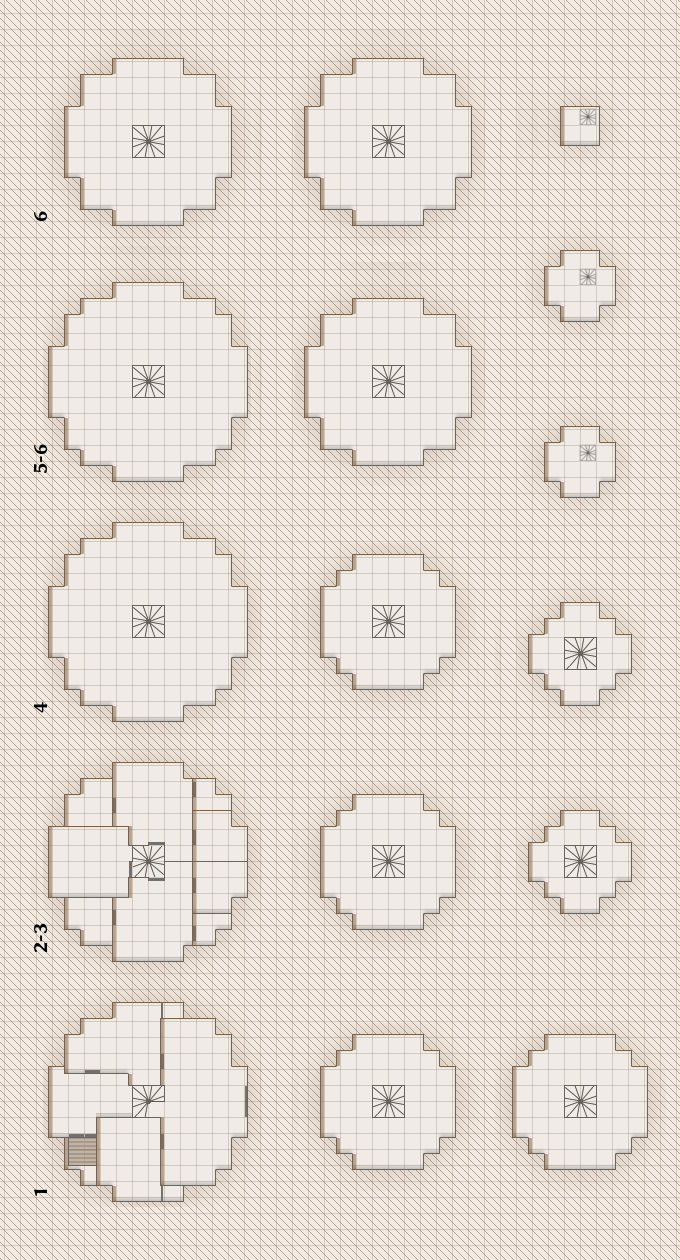
\includegraphics[width=12cm]{Maps/TourMage2.png}
\end{figure*}

